The lower level design of the system are explained in the architecture design of the system. 

\subsection{Front-end}
\begin{figure}[ht]
    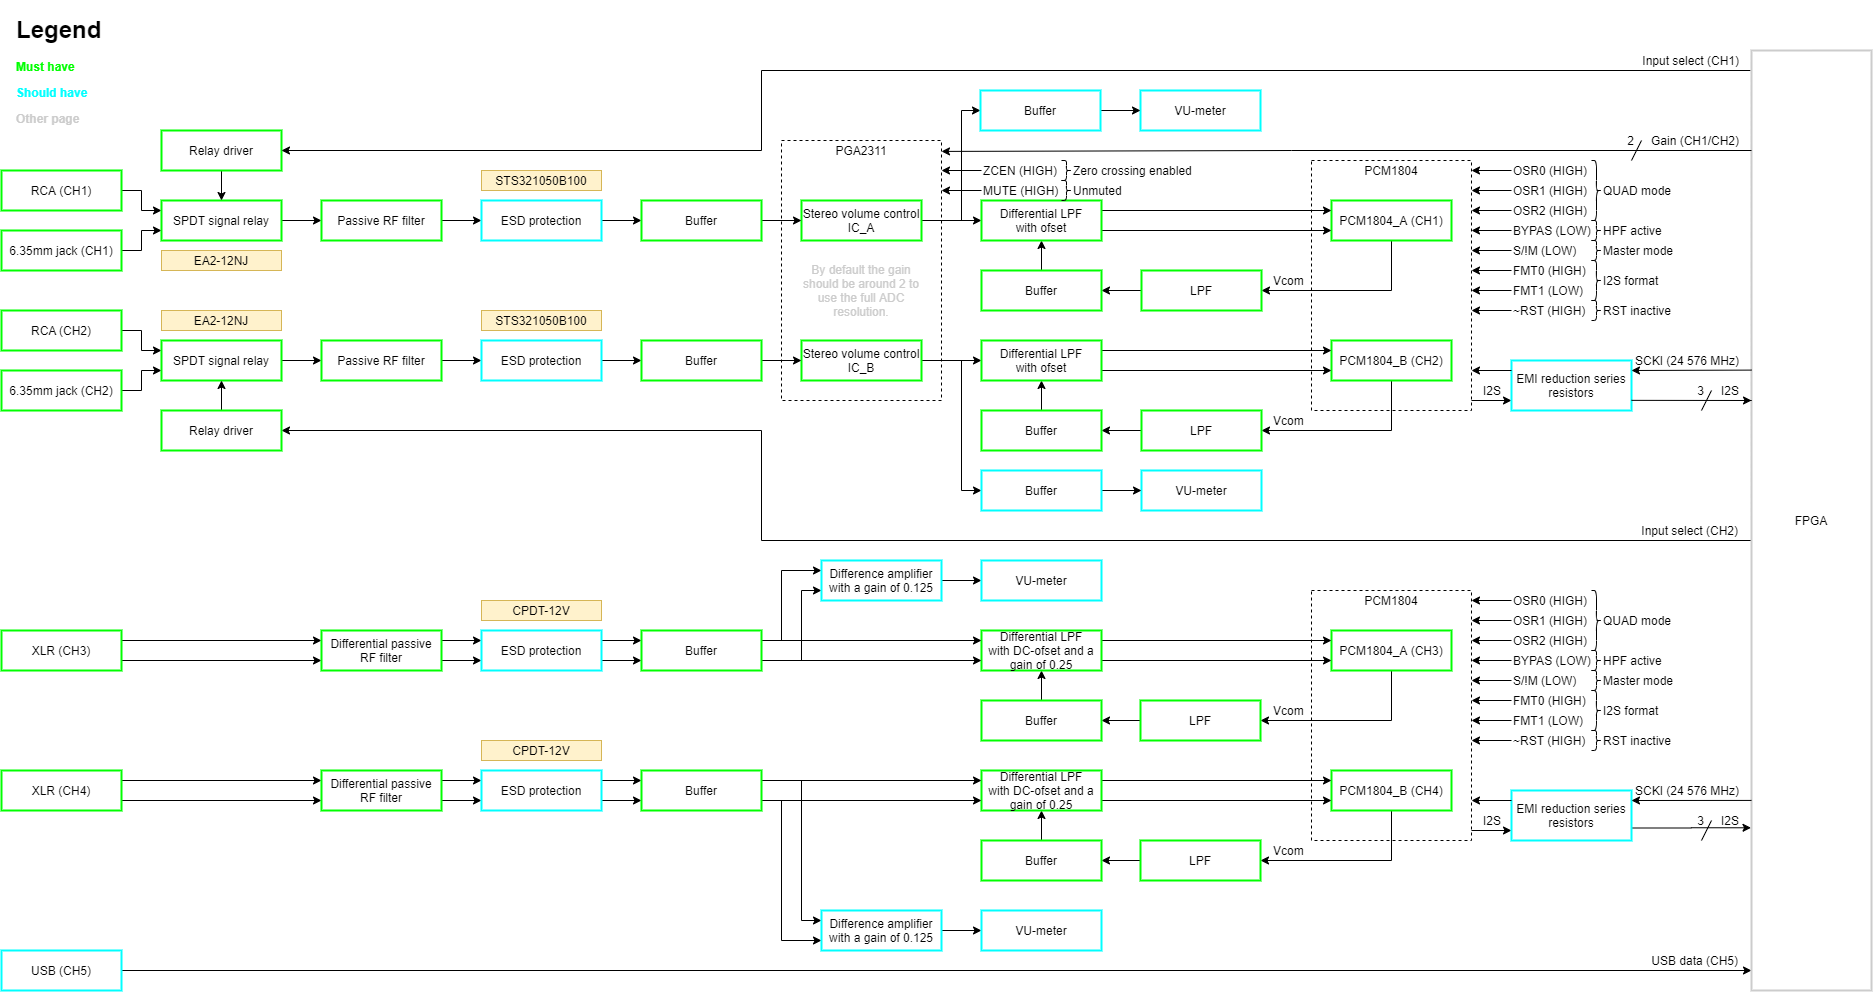
\includegraphics[width=\linewidth]{Front-end detailed.png}\\    
    \caption{Front-end architecture of audio-DSP}
    \label{fig:arch-front-end}
\end{figure}

The architecture design of the front-end of the Audio-DSP is shown in figure \ref{fig:arch-front-end}. The heart of the front-end consists of two stereo ADCs, although they are not necessarily used in stereo, and it is up to the user to choose how to utilize them. In essence, the audio DSP's front-end can be seen as four separate mono ADCs, as they provide the user with complete flexibility in their application. If time permits, the audio DSP will also feature a USB input, allowing direct digital audio input from a computer. This eliminates the need for digital-to-analog conversion by the computer's DAC and analog-to-digital conversion by the audio DSP. In theory, this USB input should offer the highest audio quality.

CH1 and CH2 each have a DPDT relay that enables the user to select between RCA or jack inputs. CH1 and CH2 are not required to use the same connector type, providing maximum flexibility to the user.

Following the input section, there are RC low-pass filters that effectively suppress high-frequency RF noise, as subsequent stages are less efficient in this regard. ESD protection diodes are then employed to divert excessive incoming voltage during an electrostatic discharge event to the system's power rails. The current during an ESD event is limited by the resistor or the RC filter.

After the RC filter and ESD protection, the signal is buffered to ensure that the preceding and subsequent stages do not interfere with each other.

The unbalanced channels, CH1 and CH2, are equipped with a volume control IC that can amplify or attenuate the incoming signal based on user preferences. This ensures optimal utilization of the ADCs' voltage range, enhancing audio quality. This volume control is particularly useful when using a guitar, as the output voltage of a guitar depends heavily on the type of guitar and playing style.

CH1 to CH4 are equipped with VU meters to visualize the amplitude of the incoming signal and detect any clipping. This information can be used to adjust the gain of the volume controller on CH1 and CH2. Each VU meter has buffers, not necessarily due to low input impedance, but primarily to minimize the surface area of current loops for sensitive signals. These buffers isolate the sensitive signal from the VU measurement.

Just before the actual ADCs, there is a differential active low-pass filter that serves as an anti-aliasing filter for the ADCs. This same LPF provides the audio signal with a DC offset voltage equal to half of the reference voltage of the used ADCs. This way, the audio signal is superimposed around a DC offset, allowing an ADC with an asymmetric supply voltage to accurately perceive the AC voltage of the audio signal. This DC offset reference voltage is generated by the ADCs and further filtered by an RC filter and buffered by an op-amp. A differential filter is employed to utilize Kelvin connections, ensuring that the differential voltage of the audio signal is independent of the voltage across the ground plane. This is the same reason why balanced XLR connectors are commonly used in professional audio, and why CH3 and CH4 are fully differential. When explaining the PCB layout, CH1 and CH2 will also be differentially routed, utilizing various Kelvin connections. However, this will never be as effective as the fully balanced XLR channels, CH3 and CH4.

The optional USB connection, CH5, is also protected by ESD diodes and then directly connected to the FPGA, which will convert the USB signal into the desired data format.

Finally, the digitized data is sent to the FPGA through the $I^2S$ protocol, where it can be processed. Due to the relatively high data rate of the I2S data, these connections are equipped with EMI reduction resistors, which essentially form an RC filter with the capacitance of the PCB trace and the ground plane, while also acting as series terminations.

\subsection{Audio-DSP}
During the development process, we came to the conclusion that the desired system could not be realized with the chosen hardware and system requirements. This is because the first design did the processing of the effects with the Fast Fourier Transform. Because the Fast Fourier Transform (FFT) requires all the samples from a certain time window at once, it takes the time window amount of time to process. This caused the latency of the system to get so large that it would not meet the requirement of 100ms propagation delay. Other than that it would not meet the requirement, it is also very complex to design the processing of the system with the FFT.

\subsubsection{Audio-DSP top-level}
\begin{figure}[ht]
    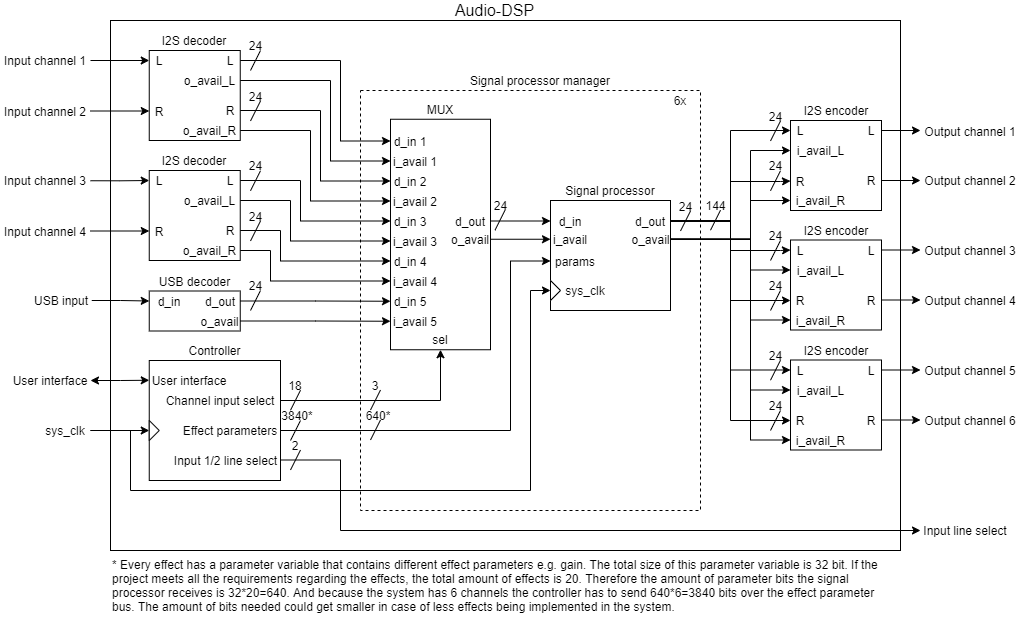
\includegraphics[width=\linewidth]{20230622_Audio-DSP design_redesign-Audio-DSP.png}\\    
    \caption{Top-level architecture of audio-DSP}
    \label{fig:arch-top}
\end{figure}

In figure \ref{fig:arch-top} you see the architecture design of the Audio-DSP. Compared to the system context diagram of the Audio-DSP the block is now much more detailed. For instance the input samplers are replaced by $I^2S$ decoders and the output signals are now encoded to $I^2S$. Because most ADCs and DACs use the $I^2S$ protocol to transfer audio data it has been chosen to use the $I^2S$ protocol. The $I^2S$ encoders and decoders each have a left and right input and output. This is because the $I^2S$ protocol transfers a stereo audio signal. But this system uses mono signals. Therefore the system inputs the mono signals on the left and right inputs. This gives the system the ability to transfer two audio channels via one $I^2S$ bus.

The MUX in each of the signal processor managers is controlled via a 3-bit select line. This select line comes from the controller. For the controller to be able to handle all the multiplexers in each signal processor manager, 3-bits $\cdot$ 6 channels = 18 bits are needed. To select the RCA or 6.35mm jack input a 2-bit line select is used.

In the signal processor block there are effects that modify the chosen input signal. These modification can be configured by using parameters. Each effect has its own parameters, e.g. a delay effect has the parameters delay time and feedback. For simplicity the size of the parameter data bus is 32-bit, which is the same size as an integer type. This makes calculations much simpler. If the project is able to meet all the requirements regarding the amount of effects, each channel would have 20 effects. Each effects then has a parameter bus of 32-bit, resulting in a parameters bus going to the signal processor block with a size equal to: $32\cdot20=640 bits$. The controller needs to send all the parameters to all the signal processors, as there are six channels the amount of data the controller needs to send over the parameters bus is equal to $640\cdot6=3840 bits$. 

To make sure that the signal processor modifies the input sample correctly it is necessary to have an input and output available bit that notifies the next effect block that the data is ready to be modified. 

% In order for the signal processor to modify the signal with various digital effects, memory is needed. This memory is stored inside the signal processor block itself. To access and modify the memory some kind of communication protocol had to be chosen in order for the controller to configure the effect parameters. For this a register based memory has been chosen.

% Looking at the system requirements it is known that the user is able to adjust the position of each effect in the effects loop. Therefore the signal processor needs registers to store the position of each effect. The system must support at least five effects and should support at least twenty effects. Thus in order to fulfill all the requirements the signal processor should be able to position twenty effects. For this we would need at least 5 bits at each position. The various effects available to the user have configurable parameters. Therefore each effect also needs a register in the signal processor block. Also the equalizer settings are adjustable by the user. This means the equalizer also has a register with data.

% The size of the registers can be very large. But to make the communication to the signal processor intuitive the registers will be limited to a maximum amount of bits. In order to choose the most efficient register size the registers should use most of its bits. The size of the register is of no importance for the effect and equalizer parameters as the size only affects the resolution of the parameters. But for the position register 5-bits per position are needed. Thus the register should be dividable by 5 in order to use the most of the registers bits. As there are 20 positions it is chosen to have four position registers with 5 positions (see figure \ref{fig:reg-position}).
% This means the register size will be 25 bits.

% \begin{figure}[ht]
%     \centering
%     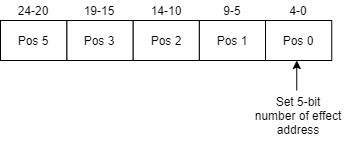
\includegraphics[width=0.4\textwidth]{Position register design}
%     \caption{Effect loop position 0 to 4 register}
%     \label{fig:reg-position}
% \end{figure}

% Now that the register size has been defined we need to define the amount of registers needed. The system has 20 effects, therefore 20 effect parameter registers. Each effect needs to be positioned in the position registers which there are four of. Then the equalizer and volume registers are left. when using 5 bits for selecting the registers we would be able to access up to 32 registers. This means that there are $32 - (20 + 4) = 8$ registers left for the equalizer and volume parameters. That is more than enough for these registers.

% Thus the data bus will be 25 bits and the register selector line will be 5 bits. With these two lines every register can be accessed by the controller. Now the memory needs to know if the data needs to be read or written. This is indicated by the R/W signal. When this signal is low the memory will be written and when the signal is high the memory will be read.

% It is undesired that every signal processor memory will be read or written constantly. Therefore each signal processor block has an enable. When this enable signal is high the memory can be read or written. This gives the controller the ability to read or write to only one signal processor memory at a time. And the ability to write multiple signal processor memories at once.

\subsubsection{Signal processor}
\begin{figure}[ht]
    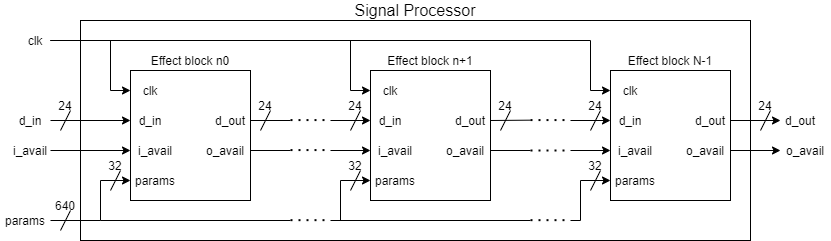
\includegraphics[width=\linewidth]{20230622_Audio-DSP design_redesign-Signal processor.png}
    \caption{Signal processor architecture}
    \label{fig:arch-signal-processor}
\end{figure}

As seen in figure \ref{fig:arch-signal-processor} all the effects are wired in series. Therefore it is needed to have some kind of handshake between each effect block to indicate if the effect can do its processing on the input data. The only thing the effect block needs to know is whether the input data is available to start the computation inside the effect. Therefore each block has an available input and output line. When the i\_avail signal goes high, the effect block starts the computation. When the computation is finished in the effect block, the o\_avail signal will be set high for a short time so the next effect block can start the computation.

\subsubsection{Effect parameters}
The implemented effects are the following:

\begin{itemize}
    \setlength\itemsep{-0.3em} %MAKES THE GAP SMALLER BETWEEN 2 ITEMS
    \item Distortion (gain)
    \item Delay
    \item Reverb
    \item Equalizer
\end{itemize}

The distortion effect works by amplifying the input signal with a gain and clipping the amplified signal at a certain level to obtain saturation. This saturation level is hardcoded in the effect. The gain can be adjusted by the user. Therefore the distortion effect only has one parameter, namely gain.

The delay effect works by adding a previous sample to the current sample creating the effect of delaying a signal. For this the delay time is a necessary parameter. The amount of time the delay lasts is configured by the feedback parameter. This simply feedbacks the output signal back to the input with a factor that causes the delayed signal to die out eventually. Another parameter used in delay effects is the mix parameter. This parameter configures the level of the delayed signal in relation to the original signal. Therefore the parameters this effects needs are: delay time, feedback and mix. 

The reverb effect works nearly identical to the delay effect but it has a feedback loop that causes the signal to decay over time. This results in the effect of reverberation. The effect can be heard in large empty rooms when you for instance clap with your hands and hear the clap reflect back from the walls. To emulate this effect the necessary parameters are the length of the reverb, which represents how long it takes for the signal to decay. Another parameter is the size of the room that it needs to emulate. This represents the time it takes for the delayed signal to reverb back from the walls. Thus the reverb effect has two parameters: length and size.

To implement the equalizer effect there are different approaches. As explained in the beginning of this chapter the first approach was to implement the effects with FFT, which would make the implementation of an equalizer much easier as you could simply modify the magnitudes of every frequency in the transformed spectrum to your liking. But because this approach has been canceled another very powerful and extremely fast mathematical method is chosen to implement the equalizer effect. The chosen method is state-space. With state-space a multiple order system can by simplified into multiple first order equations. With state-space a physical system can be represented by a set of inputs and outputs with a set of state variables related by first-order differential equations. 

Making an equalizer effect can be seen as adding up different band-pass filters. Thus to make the equalizer filter it is much simpler to represent a band-pass filter with state-space and change the state variables according to the desired frequency of the band-pass filter. To do this a physical system should be converted to state-space. The simplest system for making a band-pass filter in electronics is by having a low-pass filter in series with a buffer and a high-pass filter (see figure \ref{fig:bpf-circuit}). The calculations needed to achieve the state-space notation of this circuit can be seen in appendix ???.

\begin{figure}[ht]
    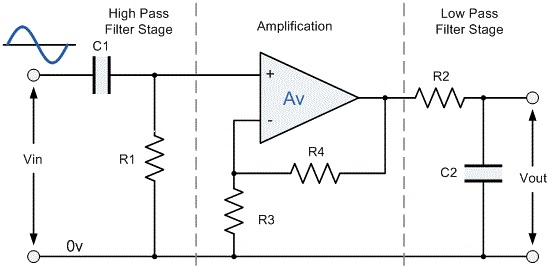
\includegraphics[width=\linewidth]{BandPassFilter_circuit.jpg}
    \caption{Band-pass filter circuit with $f_{resonance}=\frac{1}{2\pi RC}\ where\ C=C1=C2,\ R=R1=R2,\ R3=\infty\Omega\ and\ R4=0\Omega$}
    \label{fig:bpf-circuit}
\end{figure}

By having multiple band-pass filters with different cut-off frequencies the frequency spectrum is divided into individual bands, like and equalizer. The interval between these filter bands is normally described in octaves. Most commonly each filter bank is positioned at each octave as seen in figure \ref{fig:filter-banks-octave}. The shown filter bands have quite a large roll-off of approximately 40 per decade. Which means this system has band-pass filters of the fourth order. The simple band-pass circuit that this system uses is a first order band-pass filter, which therefore has a roll-off of 20dB per decade. 

\begin{figure}[ht]
    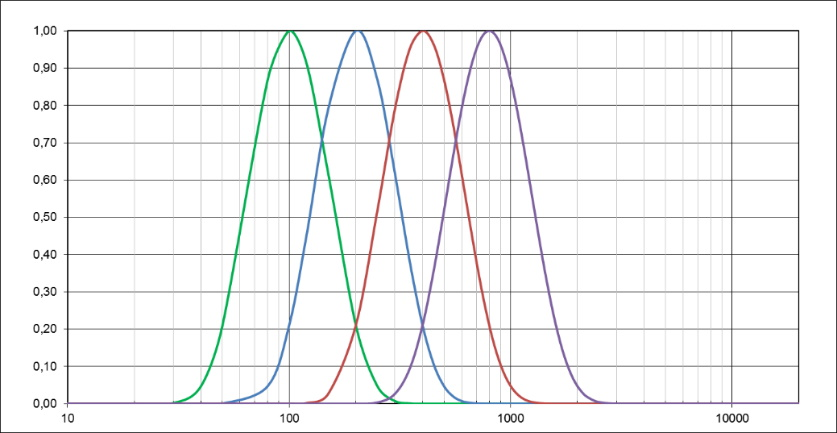
\includegraphics[width=\linewidth]{filter-banks-centered-at-octave.jpg}
    \caption{four symmetrical band-pass filters centered at each octave}
    \label{fig:filter-banks-octave}
\end{figure}

It is chosen that for simplicity of the design that the band-pass filters cross their neighboring band-pass filter at approximately -6dB. This results in a smooth transition between the band-pass filters. To achieve this the neighboring band-pass filter should have a resonance frequency that is two octaves higher than the current one.

The system has a frequency range of 20Hz to 20KHz. It is unnecessary to set the resonance frequency of the two outer band-pass filters to these outer ranges of the spectrum as these frequencies cannot be heard by most humans. Therefore it is chosen to choose the outer band-pass filter frequencies such that the magnitude at the outer ranges of the spectrum is also -6dB. Thus the most left band-pass filter has a resonance frequency that is an octave higher than the lowest frequency, $2\cdot20Hz=40Hz$. And the most right band-pass filter has a resonance frequency that is an octave lower than the highest frequency, $\frac{1}{2}\cdot20KHz=10KHz$.

Now that the outer resonance frequencies are known it is possible to calculate how many band-pass filters are able to fit between these frequencies. It is known that the distance between the resonance frequencies of neighboring band-pass filters is two octaves. The equation for computing the factor to equally distribute the resonance frequencies is as follows: 

\begin{equation}
    factor=\sqrt[N-1]{\frac{f_{high}}{f_{low}}}
\end{equation}

The value that is unknown in N. So the equation for N is as follows: 

\begin{equation}
    N=\frac{\ln\frac{f_{high}}{f_{low}}}{\ln{factor}}+1\rightarrow N=\frac{\ln\frac{10KHz}{40Hz}}{\ln{4}}+1\approx 5
\end{equation}

So with with a distance of two octaves between each band it is possible to have 5 band-pass filters within the frequency spectrum. The resulting resonance frequencies of the band-pass filters are thus: 

\begin{table}[h!]
    \centering
    \begin{tabular}{|c|c|c|}
        \hline
        \# & Resonance frequency [Hz]\\
        \hline
        1 & 40\\
        \hline
        2 & 160\\
        \hline
        3 & 640\\
        \hline
        4 & 2560\\
        \hline
        5 & 10240\\
        \hline
    \end{tabular}
    \caption{Band-pass filter resonance frequencies}
    \label{table:bpf-filters-frequencies}
\end{table}

The user is able to adjust the magnitude of each band-pass filter. This is done by adjusting the gain. So the parameter that is needed for the equalizer effect is gain for each band-pass filter. As the parameters size is 32 bits and there are 5 band-pass filters there can be $\lfloor\frac{32}{5}\rfloor=6\ bits$ available for each band-pass filter its gain parameter. This causes the parameter register to have two unused bits, which will be set to reserved.

\begin{table}[h!]
    \centering
    \begin{tabular}{|c|c|c|c|}
        \hline
        MSB & LSB & Parameter & Description\\
        \hline
        5 & 0 & Gain\_f0 & Specify magnitude of 40Hz frequency ranging from -32dB to 31dB with steps of 1dB\\
        \hline
        11 & 6 & Gain\_f1 & Specify magnitude of 160Hz frequency ranging from -32dB to 31dB with steps of 1dB\\
        \hline
        17 & 12 & Gain\_f2 & Specify magnitude of 640Hz frequency ranging from -32dB to 31dB with steps of 1dB\\
        \hline
        23 & 18 & Gain\_f3 & Specify magnitude of 2560Hz frequency ranging from -32dB to 31dB with steps of 1dB\\
        \hline
        29 & 24 & Gain\_f4 & Specify magnitude of 10240Hz frequency ranging from -32dB to 31dB with steps of 1dB\\
        \hline
        31 & 30 & Res & Reserved\\
        \hline
    \end{tabular}
    \caption{Equalizer effect parameter register}
    \label{table:eq-effect-parameters}
\end{table}

% The signal processor has to load a new sample into the effect loop and the previous modified sample to the output on the sample frequency. The sample frequency of the Audio-DSP is 192kHz. This means that the signal processor has $\frac{1}{192 \cdot 10^3} \approx 5 \mu s$ to process the sample. With a clock of 50MHz the sample must be modified and loaded into the output within $\frac{50 \cdot 10^6}{192 \cdot 10^3}=260$ clock ticks.

% When a sample has been loaded into the signal processor, it is fed into the effect processor manager (see figure \ref{fig:arch-signal-processor}). The effect processor manager houses multiple effects processor in series. The sample will go through these effect processors. Each effect processor can be configured to be a certain effect (see figure \ref{fig:arch-effect-processor}). Because the system has at least twenty effects, the amount of bits the selector needs is 5 bits.

% Each effect modifies the signal by applying a transfer function to the sample. The variables in that transfer function are configured by the user via the user interface. Therefore the effect processors needs to get the variables from the controller block, which gets the variables from the register bank. After the sample has gone through all the effect processors the modified sample waits before it is shifted out of the signal processor. 

\subsection{Back-end}
The architecture design of the back-end of the Audio-DSP is shown in figure \ref{fig:arch-back-end}. The processed data is sent from the FPGA to the DACs via the I2S protocol. The back-end consists of three stereo DACs, which, like the front-end, can be used as six separate mono channels depending on the user's preferences. Similar to the front-end, the I2S connections in the back-end are equipped with EMI reduction resistors due to the relatively high data rate.

Immediately after the DACs, differential low-pass filters are placed, serving as reconstruction filters. Finally, the signal is buffered to ensure that the output signals have relatively low impedance, reducing circuit noise.

CH1 and CH2 offer the most extensive features, providing the user with maximum flexibility. In addition to the standard balanced XLR output, each output channel in these channels is also equipped with an unbalanced RCA and jack connector. The RCA and jack connectors of the same channel are interconnected and carry the exact same signal. The output signal is always present on all outputs of that channel, as it does not adversely affect the system's performance. This way, the user does not need to consider whether a particular output connector has a signal or not. The connectors will be equipped with a small series resistor to minimize phase shift caused by the capacitance of the cables used, significantly improving system stability.

\begin{figure}[ht]
    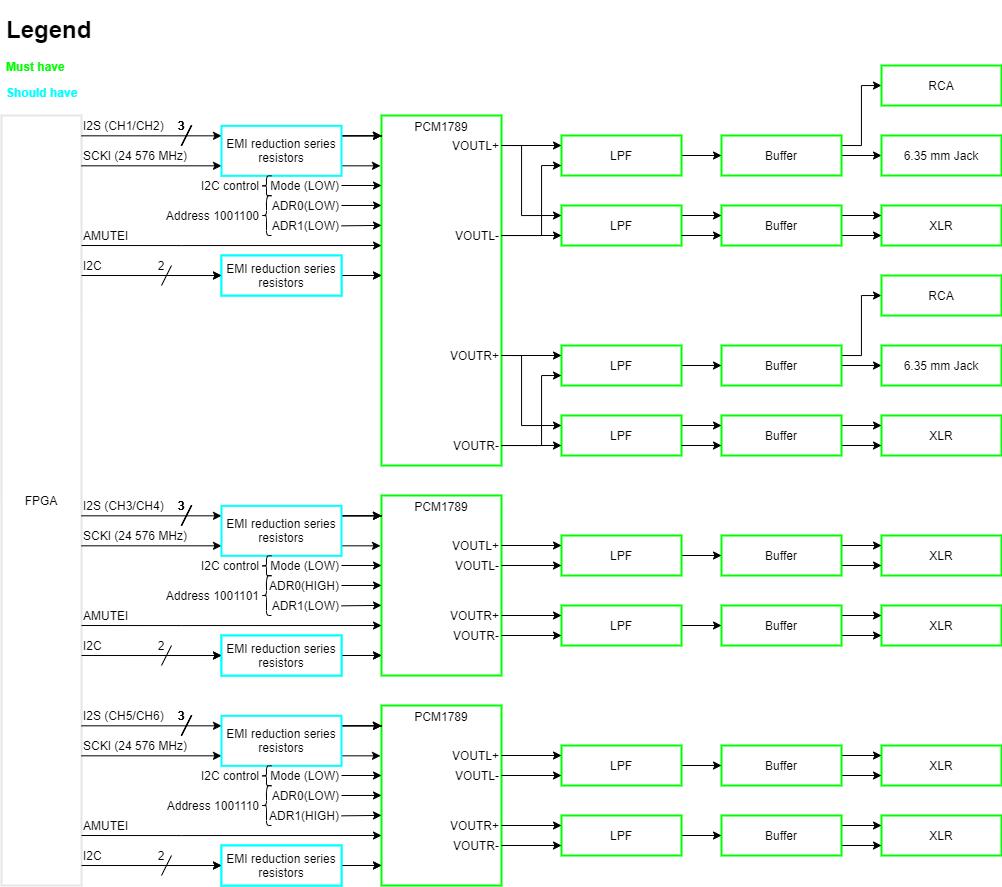
\includegraphics[width=\linewidth]{Back-end detailed.png}\\    
    \caption{Back-end architecture of audio-DSP}
    \label{fig:arch-back-end}
\end{figure}

\subsection{Power supplies}
The architecture design of the power supplies of the Audio-DSP is shown in figure \ref{fig:arch-power-supply}. The power supply section is composed of various power supplies. The ADCs and DACs impose high demands on the power supply since their analog voltages are directly referenced to the supply voltage. If the supply voltage of the analog components were to fluctuate due to potential power ripple, the digitized values from the ADCs could deviate by one or more bits. The same applies to the DACs, as the reconstructed analog voltage is directly dependent on the power supply voltage of the analog part of the DACs. To ensure that the noise caused by power fluctuations of the ADCs and DACs is smaller than the quantization error, very high requirements are set for these power supplies.

Since the availability of linear voltage regulator ICs is limited, and at the time of writing, no IC met these stringent requirements, it was decided to design and create discrete low-noise voltage regulators. Discrete designs offer the potential for much better performance than available ICs.

Similar to the ADCs and DACs, the op-amps also have high demands on power supply ripple, and therefore, comparable discrete low-noise linear regulators are used for them.

The digital side of the ADCs and DACs has much lower demands on power supply ripple, but datasheets recommend the use of linear voltage regulators for optimal performance. Hence, standard low dropout (LDO) linear voltage regulators will be used for this purpose. Discrete designs are overly emphasized for these applications.

To limit power losses and heat dissipation in the audio DSP, switching converters are used wherever possible due to their high efficiency. Buck converters are placed before the linear voltage regulators to pre-regulate the voltage, reducing the voltage drop across the linear voltage regulators and thus reducing the power dissipation.

The FPGA and signal relay are powered by a 12V buck converter. The standard power requirement for the FPGA is 12V at 2A, and to provide additional margin, our 12V power supply will be designed for a minimum of 3A to ensure sufficient current delivery and voltage stability.

The required negative power supply voltage is generated by a single-ended primary-inductor converter (SEPIC). This choice was made due to the ability to generate a negative power supply voltage, low voltage ripple, and high efficiency. The SEPIC receives 12V as an input voltage from a buck converter because the input voltage range of SEPIC converters is generally limited. The same buck converter used to power the FPGA and signal relay can be utilized for this purpose.

Ultimately, all power supplies are fed from an externally sourced 24V power supply for safety reasons. A 24V power supply was chosen because it was the most cost-effective at the time of writing. The voltage does not need to be exactly 24V since it will be further regulated by various switching regulators.

\newpage

\begin{figure}[!h]
    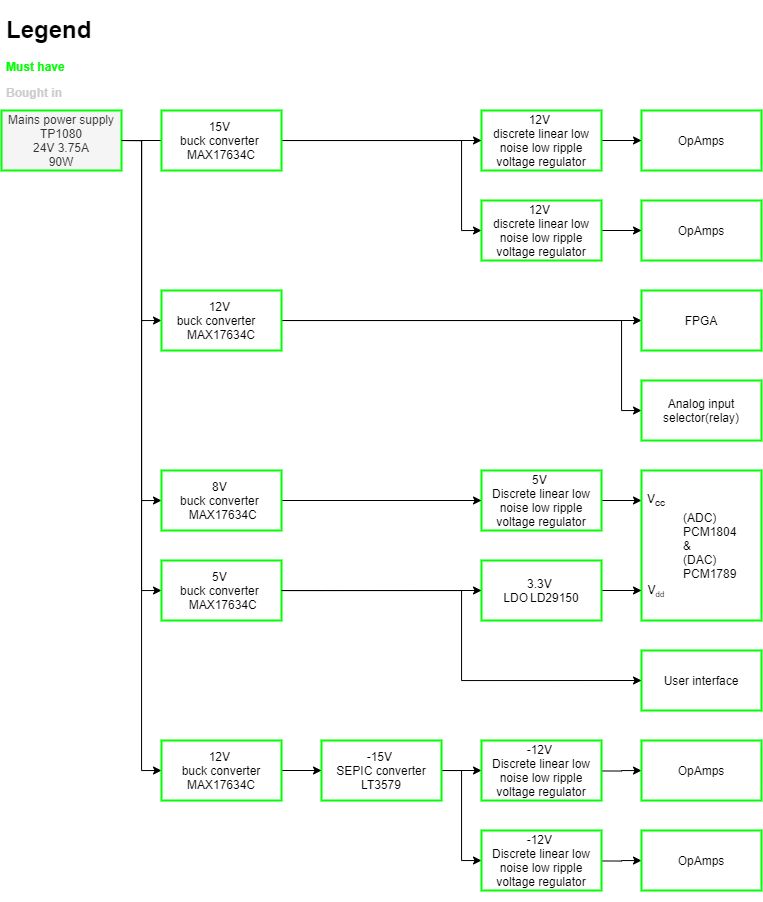
\includegraphics[width=\linewidth]{Power supply detailed.png}\\    
    \caption{Power supply architecture of audio-DSP}
    \label{fig:arch-power-supply}
\end{figure}

\par
